\documentclass[12pt]{article} %Tipo de documento

\usepackage[utf8]{inputenc}	%Codificación
\usepackage[spanish]{babel} %Idioma
\usepackage{fancyhdr, graphicx, parskip}
\usepackage[margin=1in]{geometry} %para el identado de párrafos
\usepackage{indentfirst}%para el identado de párrafos
\usepackage{array}%Tamaño de celdas
\usepackage{blindtext}%Enumeraciones

\renewcommand{\headrulewidth}{0pt}
\pagestyle{empty}


\fancyhead[L]{
	
\includegraphics[width=2cm]{images/unam.jpg}
}
\fancyhead[R]{
	
\includegraphics[width=2cm]{images/FI.jpg}
}
\fancyfoot[C]{}

\title{Propuesta de proyecto final}
\author{Gabriel, Max, Fer}
\date{\today}

\begin{document}
	\begin{titlepage}
		\thispagestyle{fancy}
		\centering
		{\bfseries - \par}
		\vspace{1cm}
		{\bfseries\LARGE UNIVERSIDAD NACIONAL AUTÓNOMA DE MÉXICO \par}
		\vspace{1cm}
		{\bfseries\LARGE Facultad de Ingeniería \par}
		\vspace{1cm}
		{\bfseries\LARGE Computación Gráfica e Interacción Humano Computadora \par}
		\vspace{1cm}
		{\bfseries\LARGE Ing. Arturo Pérez de la Cruz \par}
		\vspace{1cm}
		{\bfseries\LARGE Propuesta de proyecto final \par}
		\vspace{1cm}
		{\bfseries\LARGE Gabriel Rojas Méndez \par}
		{\bfseries\LARGE Fernanda Jiménez \par}
		{\bfseries\LARGE Max \par}
		\vspace{1cm}
		{\bfseries\LARGE Fecha de entrega: 20 de marzo de 2020 \par}
		\vspace{1cm}
		{\bfseries\LARGE Semestre 2020-2 \par}
	\end{titlepage}
	
	
	\newpage
	
	\section{Descripción general}
	
	\setlength{\parindent}{1.0cm}
	Recorrido virtual de un entorno jurásico basado en voxel art, incluyendo elementos que simulen un parque temático. 
	Tendrá dinosaurios, jaulas, vegetación e iluminación para simular el ambiente virtual. 
	Se incluirá una cámara en tercera persona para nuestro avatar y una cámara aérea que será desde el helicóptero.
	\setlength{\parindent}{0.0cm}
	
	\section{Diseño de ambiente virtual}
	
	\begin{figure}[h]
		\begin{center}
			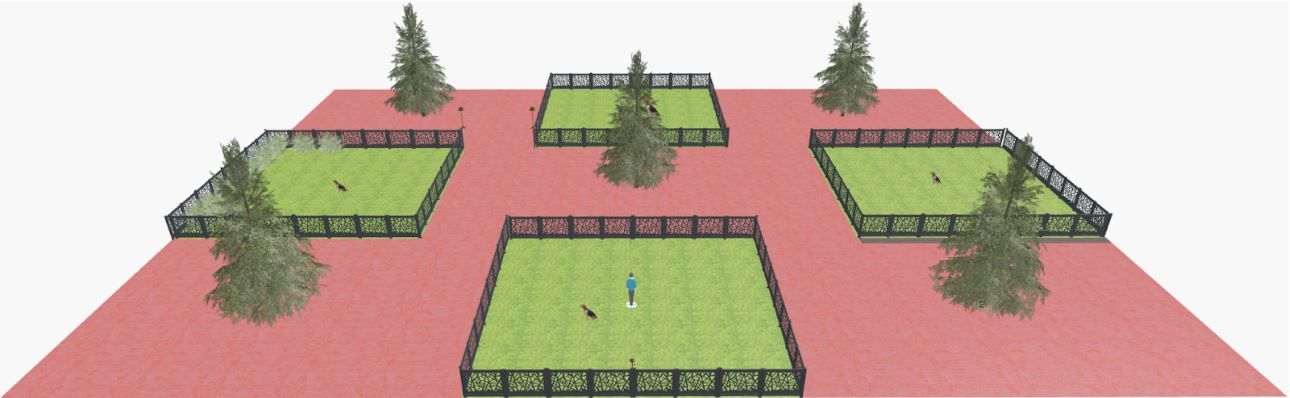
\includegraphics[scale=0.485]{images/Propuesta3D.jpg}
			\caption{Islas}
		\end{center}  		
	\end{figure}
	
	\setlength{\parindent}{1.0cm}
	Se propone una distribución de elementos similar a la Figura 1, 4 jaulas circulares, una por cada dinosaurio. 
	Cada dinosaurio estará en una pequeña isla con luces spotlight y vegetación, 
	cada isla estará conectada con caminos de concreto. 
	Los caminos tendrán lámparas que se encenderán dependiendo si es de noche o de día. 
	Cada isla contará con 2 luces spotlight, una de ellas se encenderá y apagará con teclado y la otra servirá para 
	un show de luces que igual será activada mediante teclado.
	\setlength{\parindent}{0.0cm}
	
	\begin{figure}[h]
		\begin{center}
			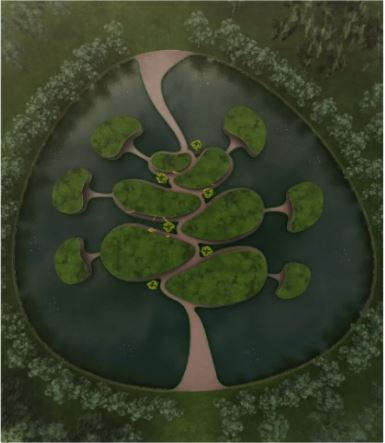
\includegraphics[scale=0.5]{images/Isla.JPG}
		\caption{Referencia de islas}
		\end{center}  		
	\end{figure}
	
	
	\newpage
	
	\section{Modelos a utilizar}
	
	\begin{center}
		\begin{tabular}{ | m{19em} | m{19em} | }
			\hline
			Nombre & Animación  \\ 
			\hline
		 	Tiranosaurio rex &
		 	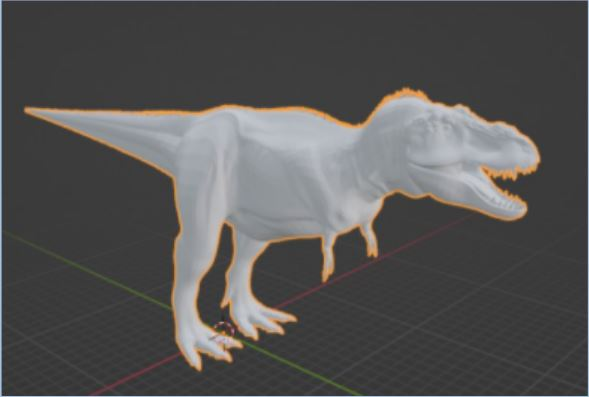
\includegraphics[scale=0.5]{images/Tiranosaurio.JPG} \\  
		 	\hline
		 	Cuello largo (Diplodocus) &
		 	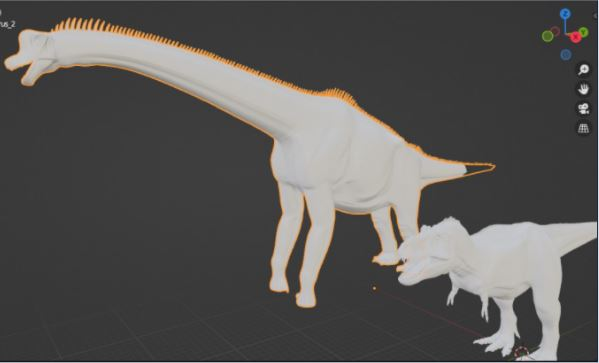
\includegraphics[scale=0.5]{images/Diplodocus.JPG} \\
		 	\hline
		 	Estegosaurio &
		 	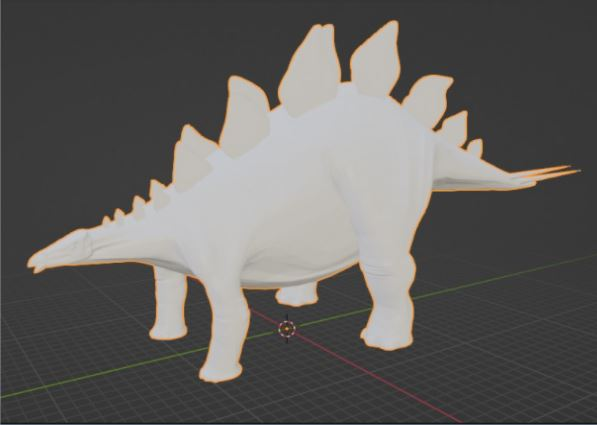
\includegraphics[scale=0.5]{images/Estegosaurio.JPG} \\  
			\hline
		\end{tabular}
	\end{center}
	\begin{center}
		\begin{tabular}{ | m{19em} | m{19em} | }
			\hline
			Nombre & Animación  \\ 
		 	\hline
		 	Velociraptor &
		 	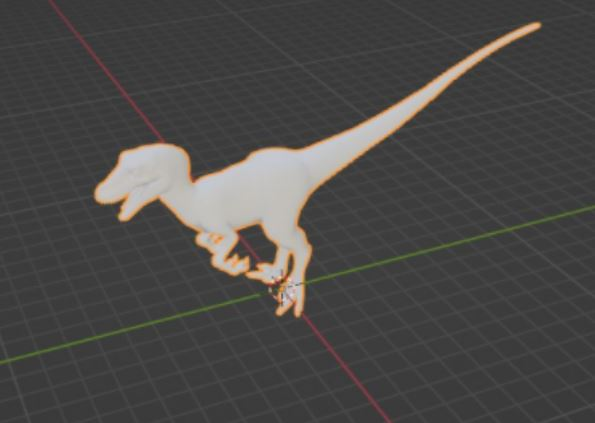
\includegraphics[scale=0.5]{images/Velociraptor.JPG} \\  
		 	\hline
		 	Helicóptero &
		 	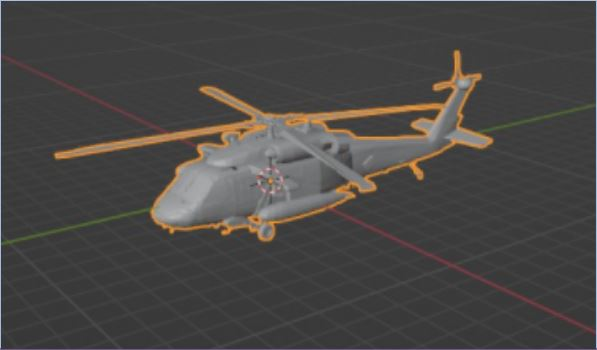
\includegraphics[scale=0.5]{images/Helicoptero.JPG} \\  
			\hline
		 	Avatar &
		 	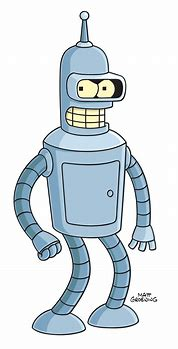
\includegraphics[scale=0.5]{images/Avatar.JPG} \\  
			\hline
		\end{tabular}
	\end{center}

	\newpage
	
	\section{Texturizado}
	
	\setlength{\parindent}{1.0cm}
	En el caso del avatar será un texturizado simple, con pantalón de mezclilla, camisa roja, gorra roja oscura. 
	Para los dinosaurios los colores serán escogidos en un futuro, sin embargo se tendrán dinosaurios con 2 colores 
	(para el lomo y la barriga) o de 1 solo color. Cada dinosaurio contará con arrugas, cicatrices y manchas.
	\setlength{\parindent}{0.0cm}
	
	\section{Elementos diferentes}
	
	\begin{itemize}
		\item[*] Dinosaurios (4)
		\item[*] Árboles (2)
		\item[*] Arbustos (2)
		\item[*] Pasto (1)
		\item[*] Agua (1)
		\item[*] Concreto (1)
		\item[*] Helicóptero (1)
		\item[*] Lámparas (1)
		\item[*] Spotlight (1)
 	\end{itemize}
 	
 	Éstos elementos serán únicos pero podrán repetirse a lo largo del escenario.
 	
 	\section{Animaciones tentativas}
	
	\begin{itemize}
		\item[*] \emph{Velociraptor:} Correr.
		\item[*] \emph{Diplodocus:} Ver a su alrededor, asegurándose que no haya presas y después bajarse a comer pasto, 
					o bien comer de un árbol.
		\item[*] \emph{Tiranosaurio:} Grito.
		\item[*] \emph{Estegosaurio:} Caminata.
		\item[*] \emph{Helicóptero:} Aceleración gradual de hélices y elevación. 
				Inclinaciones (izquerda, derecha, adelante, atrás) y giro (izquierda, derecha).
		\item[*] \emph{Avatar:} Caminata tipo Roblox.
 	\end{itemize}
 	
 	\section{Cronograma de actividades}
 	
 	\begin{center}
		\begin{tabular}{ | m{5.5em} | m{5.5em} | m{5.5em} | m{5.5em} | m{5.5em} | m{5.5em} |}
			\hline
			\# & Actividad & Fecha & Horario & Numero de Horas & Costo \\ 
			\hline
			1 &  &  &  &  & asdf \\ 
			\hline
			
		\end{tabular}
	\end{center}
	
	\section{Comentarios}
 	
	\section{Bibliografía}
	
\end{document}	